% Provenance (never printed): cycle 4 SVT, "La planete Terre, l'environnement":
% glaciers and their landforms, the cryosphere, the glaciations told; see
% sources/book1/PROVENANCE.md. Book 1, grade 8, chapter 5.
% Vocabulary guard: owns glacier; ice sheet + ice shelf + iceberg (one
% definition); sea ice; permafrost; U-shaped valley + moraine (one
% definition); ice age. "Glacial period", "interglacial" and "glacial cycle"
% belong to Book 2 g12 past-climates: here "the ice ages and the warmer times
% between them", in prose. Albedo belongs to Book 2 g10: here "reflects".
% Buoyancy and water expanding as it freezes are physics: recalled in prose.
\chapter{O gelo na Terra}\label{ch:g8:ice-on-earth}

As duas fotografias abaixo foram tiradas do mesmo lugar, numa laguna do
Alasca, com 26 anos de intervalo. Em 1990, uma larga língua de gelo descia
o \omterm{def:g1:landscapes-around-us:landform}{vale} até a água. Em 2016, o gelo tinha recuado \omterm{def:g1:landscapes-around-us:landform}{vale} acima e ficado mais
estreito; árvores e \omterm{def:g3:stones-pebbles-sand:rock}{rocha} nua ocupavam o espaço que ele tinha deixado.
Entre 1984 e 2021, as imagens de satélite mostram que a extremidade dessa
\omterm{def:g8:ice-on-earth:glacier}{geleira}, a \omterm{def:g8:ice-on-earth:glacier}{geleira} Pedersen, recuou cerca de \qty{3.2}{km}.
% ledger: commons:pedersen, uw:pedersen

\begin{omfigure}
\begin{minipage}[t]{0.49\linewidth}\centering
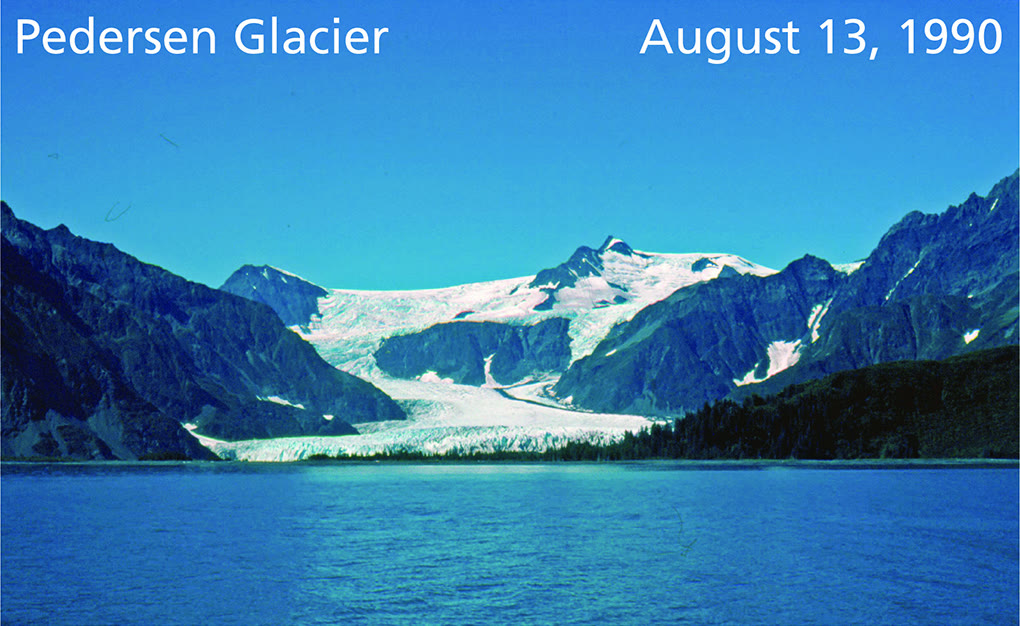
\includegraphics[width=\linewidth]{images/book1/g8-pedersen-1990.jpg}
\end{minipage}\hfill
\begin{minipage}[t]{0.49\linewidth}\centering
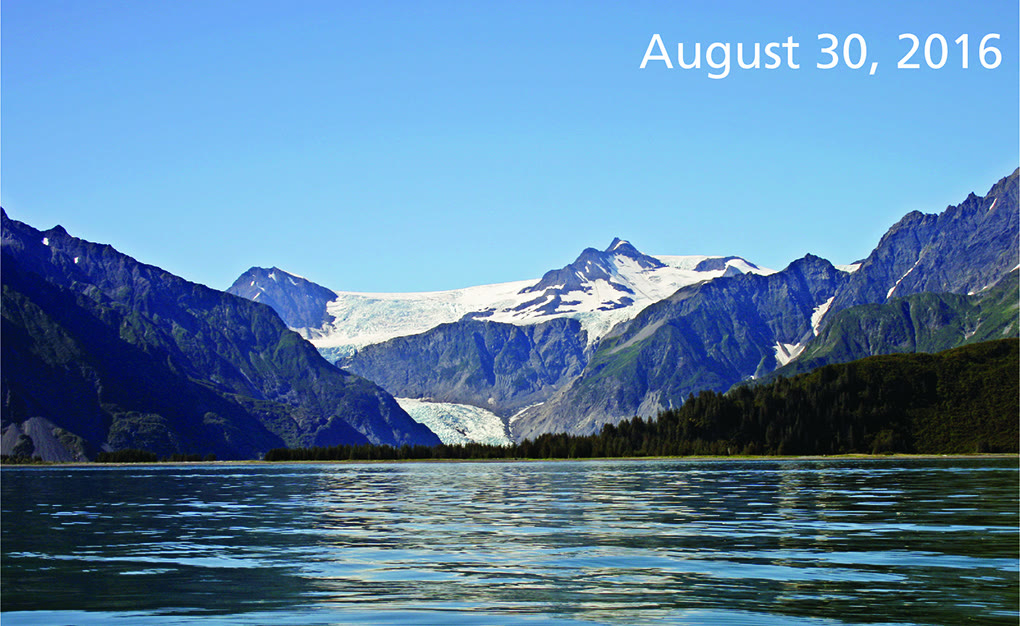
\includegraphics[width=\linewidth]{images/book1/g8-pedersen-2016.jpg}
\end{minipage}

\smallskip
{\small A \omterm{def:g8:ice-on-earth:glacier}{geleira} Pedersen, no Parque Nacional Kenai Fjords, no Alasca,
vista do mesmo lugar em 13~de~agosto~de~1990 (à esquerda, fotografia de
M.~Tetreau) e em 30~de~agosto~de~2016 (à direita, fotografia de D.~Kurtz).
U.S. National Park Service, domínio público (via Wikimedia Commons).}
% ledger: commons:pedersen
\label{fig:g8:ice-on-earth:pedersen}
\end{omfigure}

O gelo cobre hoje cerca de um décimo das terras da Terra. Ele fica nos
\omterm{def:g1:landscapes-around-us:landform}{vales} das \omterm{def:g1:landscapes-around-us:landform}{montanhas}, em dois enormes mantos sobre a Antártida e a
Groenlândia, nos \omterm{def:g2:water-on-earth:ocean}{mares} polares e, escondido, dentro do chão congelado do
extremo norte. Este capítulo olha cada um deles por vez, como o gelo
modela o \omterm{def:g4:world-physical-map:relief}{relevo}, e as épocas em que o gelo cobria muito mais a Terra do
que hoje.
% ledger: nsidc:ice-cover

\begin{recall}
A \omterm{def:g4:clouds-rain-snow:precipitation}{neve} é um tipo de \omterm{def:g4:clouds-rain-snow:precipitation}{precipitação}: cristais de gelo que crescem numa \omterm{def:g4:clouds-rain-snow:cloud}{nuvem}
e caem sem derreter (\cref{ch:g4:clouds-rain-snow}). A água corrente
desgasta o \omterm{def:g4:world-physical-map:relief}{relevo}, leva os pedaços embora e os deposita mais abaixo; um
\omterm{def:g1:landscapes-around-us:water}{rio} escava um \omterm{def:g1:landscapes-around-us:landform}{vale} (\cref{ch:g5:water-shapes-the-land}). Quando a água do
\omterm{def:g2:water-on-earth:ocean}{mar} congela, o sal fica na água em volta do gelo (\cref{ch:g8:the-oceans}).
Em física, você aprende que a água se expande quando congela, então o
gelo é menos denso que a água líquida, e que um corpo mais leve que a
água que ele desloca flutua.
\end{recall}

\section{As geleiras}

No alto das \omterm{def:g1:landscapes-around-us:landform}{montanhas}, cai mais \omterm{def:g4:clouds-rain-snow:precipitation}{neve} no inverno do que derrete no verão.
Ano após ano, a \omterm{def:g4:clouds-rain-snow:precipitation}{neve} nova enterra a \omterm{def:g4:clouds-rain-snow:precipitation}{neve} velha e a comprime. Os cristais
se compactam, o ar entre eles é espremido para fora, e, depois de cerca de
um ano, a \omterm{def:g4:clouds-rain-snow:precipitation}{neve} virou \emph{firn}, um material granuloso entre a \omterm{def:g4:clouds-rain-snow:precipitation}{neve} e o
gelo. Enterrado cada vez mais fundo, o firn se transforma em gelo duro e
sólido; para a maioria das \omterm{def:g8:ice-on-earth:glacier}{geleiras}, isso leva mais de cem anos.
% ledger: nsidc:firn

\begin{definition}[Geleira]\label{def:g8:ice-on-earth:glacier}
Uma \emph{geleira}\index{geleira} é uma massa de gelo, formada por \omterm{def:g4:clouds-rain-snow:precipitation}{neve} acumulada durante
muitos anos, que desce devagar por cima do terreno sob o seu próprio peso.
\end{definition}
% ledger: nsidc:glacier-def

Uma \omterm{def:g8:ice-on-earth:glacier}{geleira} tem duas partes. Na sua parte de cima, a \emph{zona de
acumulação}, cai mais \omterm{def:g4:clouds-rain-snow:precipitation}{neve} a cada ano do que derrete: a \omterm{def:g8:ice-on-earth:glacier}{geleira} ganha
gelo. Na sua parte de baixo, a \emph{zona de ablação}, derrete mais gelo a
cada ano do que cai de \omterm{def:g4:clouds-rain-snow:precipitation}{neve}: a \omterm{def:g8:ice-on-earth:glacier}{geleira} perde gelo. O gelo ganho em cima
continua descendo para substituir o gelo perdido embaixo. Se os dois se
equilibram, a ponta da \omterm{def:g8:ice-on-earth:glacier}{geleira}, a sua \emph{extremidade}, fica no mesmo
lugar.
% ledger: nsidc:glacier-zones

\begin{omfigure}
\begin{tikzpicture}[font=\footnotesize, >={Stealth[length=2mm]}, xscale=1.08]
  % bedrock
  \fill[black!13] (0,4.6) -- (2,3.9) -- (4,3.0) -- (6,2.0) -- (8,1.1)
    -- (10,0.45) -- (11,0.3) -- (13,0.15) -- (13,-0.5) -- (0,-0.5) -- cycle;
  % the ice body, two zones
  \begin{scope}
    \clip (0,5.5) -- (2,4.9) -- (4,4.0) -- (6,2.9) -- (8,1.8) -- (9.4,0.95)
      -- (10,0.45) -- (8,1.1) -- (6,2.0) -- (4,3.0) -- (2,3.9) -- (0,4.6) -- cycle;
    \fill[omIce] (0,-1) rectangle (5,6);
    \fill[omSea!85] (5,-1) rectangle (11,6);
  \end{scope}
  \draw[black!60] (0,5.5) -- (2,4.9) -- (4,4.0) -- (6,2.9) -- (8,1.8)
    -- (9.4,0.95) -- (10,0.45);
  \draw[black!70, line width=0.6pt] (0,4.6) -- (2,3.9) -- (4,3.0) -- (6,2.0)
    -- (8,1.1) -- (10,0.45) -- (11,0.3) -- (13,0.15);
  % snowline
  \draw[dashed, black!70] (5,2.5) -- (5,4.15);
  \node[anchor=south] at (5,4.15) {queda de neve = derretimento};
  % snowflakes and melting
  \foreach \x/\y in {0.5/6.1, 1.3/5.8, 2.1/5.5, 2.9/5.1, 3.7/4.8, 0.9/6.6, 1.7/6.3, 2.5/6.0, 3.3/5.6, 4.1/5.2}
    \node[omCold] at (\x,\y) {$\ast$};
  \foreach \x/\y in {6.4/2.8, 7.2/2.35, 8.0/1.9}
    \draw[omWarm, decorate, decoration={snake, amplitude=0.6mm, segment length=2mm}] (\x,\y) -- ++(0,0.6);
  % flow arrows inside the ice
  \draw[->, omDef, line width=0.9pt] (1.0,4.72) -- (2.2,4.30);
  \draw[->, omDef, line width=0.9pt] (3.0,3.95) -- (4.2,3.41);
  \draw[->, omDef, line width=0.9pt] (5.2,2.88) -- (6.4,2.28);
  \draw[->, omDef, line width=0.9pt] (7.2,1.84) -- (8.3,1.35);
  % moraine and meltwater
  \fill[omLithCongl] (10.15,0.42) .. controls (10.5,0.95) and (10.9,0.95) .. (11.2,0.29) -- cycle;
  \draw[omSea!60!black, line width=1.6pt] (10.05,0.38) .. controls (10.6,0.22) and (11.4,0.12) .. (12.9,0.08);
  % labels
  \node[align=center] at (1.9,7.15) {zona de acumulação:\\ a neve se acumula, a geleira ganha gelo};
  \node[align=center] at (10.0,3.3) {zona de ablação:\\ o gelo derrete, a geleira perde gelo};
  \node[align=left, anchor=west, omDef] at (4.4,1.3) {o gelo desce\\ a encosta};
  \draw[black!60] (10.0,0.5) -- (9.6,-0.1) node[below] {extremidade};
  \draw[black!60] (10.7,0.85) -- (11.3,1.4) node[above] {morena};
  \node[anchor=north east] at (12.9,0.0) {riacho de degelo};
  \node at (2.2,2.6) {rocha do substrato};
\end{tikzpicture}

{\small Uma \omterm{def:g8:ice-on-earth:glacier}{geleira} de \omterm{def:g1:landscapes-around-us:landform}{vale} vista num corte longitudinal (um esboço, fora
de escala). Acima da linha tracejada, a \omterm{def:g4:clouds-rain-snow:precipitation}{neve} se acumula mais depressa do
que derrete; abaixo dela, o gelo derrete mais depressa do que cai a \omterm{def:g4:clouds-rain-snow:precipitation}{neve}.
O gelo desce de uma parte para a outra.}
\label{fig:g8:ice-on-earth:long-section}
\end{omfigure}

Como o gelo sólido pode escorrer? Sob o peso do gelo de cima, o gelo do
fundo de uma \omterm{def:g8:ice-on-earth:glacier}{geleira} se deforma devagar, como uma camada grossa de mel
frio se espalha. A \omterm{def:g8:ice-on-earth:glacier}{geleira} também desliza sobre a \omterm{def:g3:stones-pebbles-sand:rock}{rocha} de baixo, sobre
uma película fina de água ou sobre \omterm{def:g3:stones-pebbles-sand:sand}{lama} molhada. O fundo da \omterm{def:g8:ice-on-earth:glacier}{geleira}, que
se esfrega na \omterm{def:g3:stones-pebbles-sand:rock}{rocha}, anda mais devagar que o seu topo. A maioria das
\omterm{def:g8:ice-on-earth:glacier}{geleiras} anda devagar e de maneira regular; algumas fazem de repente um
\emph{avanço brusco}. Em 1986, a \omterm{def:g8:ice-on-earth:glacier}{geleira} Hubbard, no Alasca, avançou
cerca de \qty{10}{m} por dia, e o avanço brusco mais rápido já
registrado, o da \omterm{def:g8:ice-on-earth:glacier}{geleira} Kutiah, no Paquistão, em 1953, teve uma média de
cerca de \qty{112}{m} por dia durante três meses.
% ledger: nsidc:glacier-flow, nsidc:surges

Quando uma \omterm{def:g8:ice-on-earth:glacier}{geleira} perde mais gelo embaixo do que ganha em cima, a sua
extremidade sobe de volta pelo \omterm{def:g1:landscapes-around-us:landform}{vale}: a \omterm{def:g8:ice-on-earth:glacier}{geleira} \emph{recua}. Uma \omterm{def:g8:ice-on-earth:glacier}{geleira}
que recua continua descendo a encosta, como uma esteira transportadora;
ela só derrete mais depressa do que desce. A \omterm{def:g8:ice-on-earth:glacier}{geleira} Muir, no Alasca,
enchia o seu \omterm{def:g1:landscapes-around-us:landform}{vale} inteiro até o \omterm{def:g2:water-on-earth:ocean}{mar} em 1941. Em 2004, a sua extremidade
tinha recuado \qty{12}{km}, e a superfície do gelo tinha baixado mais de
\qty{800}{m}.
% ledger: nsidc:glacier-flow, nsidc:muir

\section{Como o gelo modela um vale}

Uma \omterm{def:g8:ice-on-earth:glacier}{geleira} é uma ferramenta de \omterm{def:g5:water-shapes-the-land:erosion}{erosão} poderosa. O seu gelo congela em
volta de blocos de \omterm{def:g3:stones-pebbles-sand:rock}{rocha} solta e os arranca; as pedras presas na sua base
raspam a \omterm{def:g3:stones-pebbles-sand:rock}{rocha} de baixo como uma lixa. A \omterm{def:g8:ice-on-earth:glacier}{geleira} leva toda essa \omterm{def:g3:stones-pebbles-sand:rock}{rocha}, da
poeira fina a matacões enormes, \omterm{def:g1:landscapes-around-us:landform}{vale} abaixo, como uma esteira
transportadora, e a larga onde o gelo derrete.
% ledger: nps:u-valley

\begin{omfigure}
\begin{tikzpicture}[font=\footnotesize, >={Stealth[length=2mm]}]
  % V-shaped valley
  \fill[black!13] (0,3) -- (2.1,0.35) -- (2.5,0.35) -- (4.6,3) -- (4.6,-0.4) -- (0,-0.4) -- cycle;
  \draw[black!70, line width=0.6pt] (0,3) -- (2.1,0.35) -- (2.5,0.35) -- (4.6,3);
  \fill[omSea] (2.1,0.35) -- (2.5,0.35) -- (2.42,0.2) -- (2.18,0.2) -- cycle;
  \node[align=center] at (2.3,-0.85) {um rio escava um vale\\ estreito em V};
  % arrow
  \draw[->, line width=1pt] (5.0,1.5) -- (6.2,1.5) node[midway, above, align=center] {uma geleira\\ o enche};
  % U-shaped valley
  \begin{scope}[xshift=6.6cm]
    \fill[black!13] (0,3) .. controls (0.6,1.0) and (0.9,0.25) .. (1.6,0.2)
      -- (3.0,0.2) .. controls (3.7,0.25) and (4.0,1.0) .. (4.6,3) -- (4.6,-0.4) -- (0,-0.4) -- cycle;
    \draw[black!70, line width=0.6pt] (0,3) .. controls (0.6,1.0) and (0.9,0.25) .. (1.6,0.2)
      -- (3.0,0.2) .. controls (3.7,0.25) and (4.0,1.0) .. (4.6,3);
    \draw[dashed, black!40] (0,3) -- (2.1,0.35) -- (2.5,0.35) -- (4.6,3);
    \draw[omCold, line width=0.9pt] (0.37,2.2) -- (4.23,2.2);
    \node[omCold, anchor=south, font=\scriptsize] at (2.3,2.2) {topo do gelo, há muito tempo};
    \fill[omLithCongl] (0.75,0.95) .. controls (0.95,1.2) and (1.1,1.1) .. (1.2,0.6) -- cycle;
    \fill[omLithCongl] (3.85,0.95) .. controls (3.65,1.2) and (3.5,1.1) .. (3.4,0.6) -- cycle;
    \node[align=center] at (2.3,-0.85) {depois que o gelo vai embora: um\\ vale largo em U, encostas íngremes};
    \draw[black!60] (3.65,0.95) -- (4.85,0.6) node[right, align=left] {morena\\ lateral};
    \node[font=\scriptsize, black!55, align=center] at (2.3,1.6) {(antigo V tracejado)};
  \end{scope}
\end{tikzpicture}

{\small O mesmo \omterm{def:g1:landscapes-around-us:landform}{vale} de \omterm{def:g1:landscapes-around-us:landform}{montanha} em corte transversal, antes e depois de
uma \omterm{def:g8:ice-on-earth:glacier}{geleira} (um esboço). O gelo raspa o \omterm{def:g1:landscapes-around-us:landform}{vale} estreito do \omterm{def:g1:landscapes-around-us:water}{rio} e o
transforma numa calha larga, de fundo amplo e encostas íngremes, e deixa
cristas de detritos rochosos ao longo das suas bordas.}
\label{fig:g8:ice-on-earth:v-and-u}
\end{omfigure}

\begin{definition}[Vale em U e morena]\label{def:g8:ice-on-earth:glacial-landforms}
Um \emph{vale em U}\index{vale em U} é um \omterm{def:g1:landscapes-around-us:landform}{vale} de fundo largo e plano e encostas íngremes,
escavado por uma \omterm{def:g8:ice-on-earth:glacier}{geleira} que alargou e aprofundou um \omterm{def:g1:landscapes-around-us:landform}{vale} de \omterm{def:g1:landscapes-around-us:water}{rio} estreito
em V. Uma \emph{morena}\index{morena} é uma crista de detritos rochosos, da poeira aos
matacões, deixada por uma \omterm{def:g8:ice-on-earth:glacier}{geleira}: uma \emph{morena lateral} ao longo do
seu lado, uma \emph{morena frontal} na sua extremidade.
\end{definition}
% ledger: usgs:erratic, nps:u-valley, nps:moraines

As \omterm{def:g8:ice-on-earth:glacial-landforms}{morenas} são pistas úteis. Uma \omterm{def:g8:ice-on-earth:glacial-landforms}{morena} frontal bem abaixo num \omterm{def:g1:landscapes-around-us:landform}{vale}, sem
nenhum gelo por perto, mostra até onde a \omterm{def:g8:ice-on-earth:glacier}{geleira} chegou um dia; uma
\omterm{def:g8:ice-on-earth:glacial-landforms}{morena} lateral no alto da encosta de um \omterm{def:g1:landscapes-around-us:landform}{vale} mostra que espessura o gelo
teve um dia. Um grande matacão sozinho no meio de um campo, feito de uma
\omterm{def:g3:stones-pebbles-sand:rock}{rocha} que não se encontra em nenhum lugar por perto, é outra pista: é um
\emph{bloco errático}, uma \omterm{def:g3:stones-pebbles-sand:rock}{rocha} levada para longe do seu lugar de origem
por uma \omterm{def:g8:ice-on-earth:glacier}{geleira} e deixada para trás quando o gelo derreteu. Os blocos
erráticos vão de \omterm{def:g3:stones-pebbles-sand:pebble}{seixos} a blocos maiores que uma casa.
% ledger: nps:moraines, usgs:erratic

\begin{inthefield}[Ler um vale modelado pelo gelo]
Num passeio na \omterm{def:g1:landscapes-around-us:landform}{montanha}, ou numa fotografia de um \omterm{def:g1:landscapes-around-us:landform}{vale} de \omterm{def:g1:landscapes-around-us:landform}{montanha},
observe a forma do \omterm{def:g1:landscapes-around-us:landform}{vale} em corte transversal: um V estreito, ou um U largo
de paredes íngremes? Procure no fundo do \omterm{def:g1:landscapes-around-us:landform}{vale} longas cristas de pedras e
de terra misturadas, que correm ao longo das suas encostas ou de um lado a
outro: elas podem ser \omterm{def:g8:ice-on-earth:glacial-landforms}{morenas}. Procure grandes matacões que não combinam
com a \omterm{def:g3:stones-pebbles-sand:rock}{rocha} em volta, e superfícies de \omterm{def:g3:stones-pebbles-sand:rock}{rocha} lisas riscadas por longas
linhas paralelas. Fique nas trilhas, mantenha-se longe das bordas das
encostas íngremes e do próprio gelo, e desenhe o que você vê no seu
caderno.
\end{inthefield}

\section{Mantos de gelo, plataformas de gelo e icebergs}

As maiores massas de gelo da Terra não ficam nos \omterm{def:g1:landscapes-around-us:landform}{vales} das \omterm{def:g1:landscapes-around-us:landform}{montanhas}: elas
cobrem terras inteiras. O \omterm{def:g8:ice-on-earth:ice-sheet}{manto de gelo} da Antártida se estende por quase
\num{14}~milhões~de~\unit{km^2} e tem quase \qty{4.9}{km} de espessura no seu ponto mais espesso.
O \omterm{def:g8:ice-on-earth:ice-sheet}{manto de gelo} da Groenlândia cobre cerca de \num{1.7}~milhão~de~\unit{km^2},
quatro quintos da ilha, e tem mais de \qty{3}{km} de espessura. Juntos,
eles guardam mais de 99~\% do gelo sobre terra, e mais de dois terços de
toda a \omterm{def:g2:water-on-earth:salt-fresh}{água doce} da Terra.
% ledger: nsidc:ice-sheets

\begin{definition}[Manto de gelo, plataforma de gelo e iceberg]\label{def:g8:ice-on-earth:ice-sheet}
Um \emph{manto de gelo}\index{manto de gelo} é uma massa de gelo que cobre mais de
\qty{50000}{km^2} de terra, como uma cúpula enorme que se espalha para
fora em todas as direções. Onde o gelo que escorre da terra chega ao \omterm{def:g2:water-on-earth:ocean}{mar} e
continua flutuando sobre ele, ainda ligado ao gelo de trás, ele forma uma
\emph{plataforma de gelo}\index{plataforma de gelo}. Um \emph{iceberg}\index{iceberg} é um grande bloco de gelo, com mais de \qty{5}{m}
de largura, que se soltou de uma \omterm{def:g8:ice-on-earth:glacier}{geleira} ou de uma plataforma de gelo e
flutua no \omterm{def:g2:water-on-earth:ocean}{mar}.
\end{definition}
% ledger: nsidc:ice-sheets, nsidc:ice-shelves, nsidc:iceberg

\begin{omfigure}
\begin{minipage}[c]{0.5\linewidth}\centering
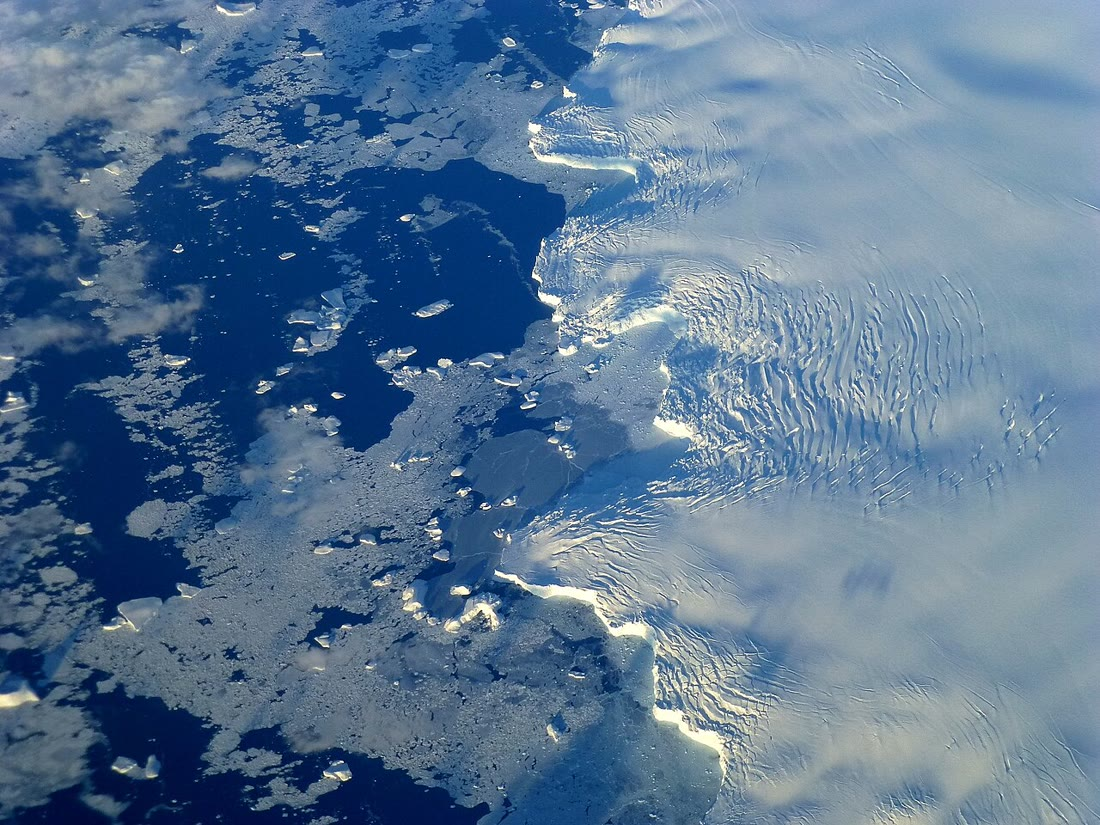
\includegraphics[width=\linewidth]{images/book1/g8-ice-shelf-edge.jpg}
\end{minipage}\hfill
\begin{minipage}[c]{0.46\linewidth}\raggedright
{\small A borda de uma \omterm{def:g8:ice-on-earth:ice-sheet}{plataforma de gelo} perto da ilha Adelaide, ao largo
da Península Antártica, vista de um avião em 28~de~outubro~de~2012. O gelo
branco, espesso e enrugado, à direita, é a \omterm{def:g8:ice-on-earth:ice-sheet}{plataforma de gelo}; à esquerda,
pedaços quebrados de \omterm{def:g8:ice-on-earth:sea-ice}{gelo marinho} mais fino flutuam na água escura. NASA,
Operation IceBridge (domínio público, via Wikimedia Commons).}
\end{minipage}
% ledger: commons:ice-shelf
\label{fig:g8:ice-on-earth:ice-shelf}
\end{omfigure}

A água presa nos \omterm{def:g8:ice-on-earth:ice-sheet}{mantos de gelo} veio do \omterm{def:g2:water-on-earth:ocean}{oceano}: ela evaporou, caiu como
\omterm{def:g4:clouds-rain-snow:precipitation}{neve} e se acumulou sobre a terra. Se todo o gelo da Groenlândia
derretesse, o \omterm{def:g2:water-on-earth:ocean}{mar} subiria cerca de \qty{7.4}{m}; se todo o gelo da
Antártida derretesse, cerca de \qty{58}{m}. Todas as \omterm{def:g8:ice-on-earth:glacier}{geleiras} de \omterm{def:g1:landscapes-around-us:landform}{montanha}
do mundo, mais de \num{200000}, acrescentariam menos de meio metro.
% ledger: nsidc:ice-sheets, nsidc:ice-cover

\begin{omfigure}
\begin{tikzpicture}
\begin{axis}[omrecord, xbar, width=10.5cm, height=3.6cm, xmin=0, xmax=68,
  bar width=9pt, ytick=data, symbolic y coords={geleiras,Groenlandia,Antartida},
  yticklabels={todas as geleiras de montanha, manto de gelo da Groenlândia, manto de gelo da Antártida},
  xlabel={subida do mar se tudo derretesse (m)}, enlarge y limits=0.3,
  nodes near coords, nodes near coords style={font=\footnotesize, anchor=west, fill=white, inner sep=1.5pt},
  ymajorgrids=false]
  \addplot[fill=omIce!80!black, draw=black!60] coordinates {(0.5,geleiras) (7.4,Groenlandia) (58,Antartida)};
\end{axis}
\end{tikzpicture}

{\small Quanto o \omterm{def:g2:water-on-earth:ocean}{mar} subiria se cada tipo de gelo sobre terra derretesse
completamente (valores do National Snow and Ice Data Center; o valor das
\omterm{def:g8:ice-on-earth:glacier}{geleiras} é um limite superior, ``um pouco menos de meio metro'').}
% ledger: nsidc:ice-sheets, nsidc:ice-cover
\label{fig:g8:ice-on-earth:sea-level-bars}
\end{omfigure}

O gelo que flutua é diferente. Uma \omterm{def:g8:ice-on-earth:ice-sheet}{plataforma de gelo} ou um \omterm{def:g8:ice-on-earth:ice-sheet}{iceberg} já
flutua no \omterm{def:g2:water-on-earth:ocean}{mar}: ele já deslocou o seu próprio peso de água. Quando ele se
quebra ou derrete, o \omterm{def:g2:water-on-earth:ocean}{mar} não sobe. Mas uma \omterm{def:g8:ice-on-earth:ice-sheet}{plataforma de gelo} segura as
\omterm{def:g8:ice-on-earth:glacier}{geleiras} atrás dela, como uma rolha numa garrafa; quando a \omterm{def:g8:ice-on-earth:ice-sheet}{plataforma de
gelo} Larsen~B, na Antártida, se despedaçou em 2002, as \omterm{def:g8:ice-on-earth:glacier}{geleiras} atrás
dela aceleraram, algumas até oito vezes a sua velocidade anterior, e
despejaram mais gelo de terra no \omterm{def:g2:water-on-earth:ocean}{mar}.
% ledger: nsidc:ice-shelves

\begin{inthelab}[Gelo que flutua e gelo sobre terra]
Dentro de casa, ponha uma pedrinha em cada um de dois copos transparentes,
de modo que ela fique para fora da água quando você os encher. No
primeiro copo, faça flutuar alguns cubos de gelo na água. No segundo,
equilibre o mesmo número de cubos de gelo sobre a pedra, fora da água.
Encha os dois copos de água até o mesmo nível e marque-o com uma caneta
hidrográfica. Espere até todo o gelo derreter, e depois compare os níveis
da água com as marcas. Que copo se comporta como o \omterm{def:g2:water-on-earth:ocean}{mar} quando um \omterm{def:g8:ice-on-earth:ice-sheet}{iceberg}
derrete, e qual se comporta como o \omterm{def:g2:water-on-earth:ocean}{mar} quando um \omterm{def:g8:ice-on-earth:ice-sheet}{manto de gelo} derrete?
\end{inthelab}

\section{O gelo marinho}

O \omterm{def:g8:ice-on-earth:sea-ice}{gelo marinho} é ainda outra coisa: é o próprio \omterm{def:g2:water-on-earth:ocean}{mar}, congelado. A cada
inverno, a superfície dos \omterm{def:g2:water-on-earth:ocean}{oceanos} polares congela numa área enorme; a
cada verão, boa parte desse gelo derrete de novo. No Ártico, o gelo é
menor no fim do verão, em setembro, e maior no fim do inverno, em março.
Os satélites medem a sua \emph{extensão}, a área de \omterm{def:g2:water-on-earth:ocean}{mar} onde pelo menos
15~\% da superfície está coberta de gelo, todos os dias desde o fim dos
anos 1970.
% ledger: nsidc:sea-ice-def

\begin{definition}[Gelo marinho]\label{def:g8:ice-on-earth:sea-ice}
O \emph{gelo marinho}\index{gelo marinho} é água do \omterm{def:g2:water-on-earth:ocean}{mar} congelada: ele se forma, cresce e
derrete no próprio \omterm{def:g2:water-on-earth:ocean}{oceano}. Ele é diferente dos \omterm{def:g8:ice-on-earth:ice-sheet}{icebergs} e das \omterm{def:g8:ice-on-earth:ice-sheet}{plataformas
de gelo}, que flutuam no \omterm{def:g2:water-on-earth:ocean}{mar}, mas foram feitos de \omterm{def:g4:clouds-rain-snow:precipitation}{neve} caída sobre a terra.
\end{definition}
% ledger: nsidc:sea-ice-def

O \omterm{def:g8:ice-on-earth:sea-ice}{gelo marinho} importa muito além dos \omterm{def:g3:continents-and-oceans:poles}{polos}. A água do \omterm{def:g2:water-on-earth:ocean}{mar} aberta é
escura: ela reflete só cerca de 6~\% da luz do Sol que chega até ela e
absorve o resto. O \omterm{def:g8:ice-on-earth:sea-ice}{gelo marinho} reflete de 50 a 70~\%, e o \omterm{def:g8:ice-on-earth:sea-ice}{gelo marinho}
coberto de \omterm{def:g4:clouds-rain-snow:precipitation}{neve}, até 90~\%. Quando o gelo derrete, a água escura de baixo
absorve mais energia do Sol e esquenta, o que derrete mais gelo.
% ledger: nsidc:sea-ice-reflect

\begin{omfigure}
\begin{tikzpicture}
\begin{axis}[omrecord, width=13cm, height=5.4cm, xmin=1977, xmax=2027,
  ymin=3, ymax=8.2, xtick={1980,1990,...,2020},
  x tick label style={/pgf/number format/1000 sep={}},
  xlabel={ano}, ylabel={extensão (milhões de km$^2$)},
  legend style={at={(0.98,0.97)}, anchor=north east, draw=none, fill=white}]
  \addplot[omCold, mark=*, mark size=1.3pt, line width=0.6pt]
    table[x=year, y=extent_Mkm2] {figdata/out/grade-8-sea_ice-extent.dat};
  \addlegendentry{extensão média de setembro}
  \addplot[omWarm, dashed, line width=1pt]
    table[x=year, y=extent_Mkm2] {figdata/out/grade-8-sea_ice-trend.dat};
  \addlegendentry{linha de tendência}
  \node[font=\scriptsize, anchor=north] at (axis cs:2012,3.5) {2012};
\end{axis}
\end{tikzpicture}

{\small A extensão do \omterm{def:g8:ice-on-earth:sea-ice}{gelo marinho} do Ártico em cada setembro, 1979--2025,
e a reta que melhor acompanha os pontos. Dados: NSIDC Sea Ice Index,
versão~4 (F.~Fetterer e outros, 2025).}
% ledger: data:b1-nsidc-sea-ice (figdata/grade-8/sea_ice.py)
\label{fig:g8:ice-on-earth:sea-ice}
\end{omfigure}

Os pontos sobem e descem de um ano para o outro: o \omterm{def:g1:watching-the-weather:weather}{tempo} de cada verão
conta. Mas, ao longo dos anos, eles claramente descem. Para ver a mudança
através dos altos e baixos, os cientistas traçam uma \emph{linha de
tendência}, a reta que passa o mais perto possível de todos os pontos.
% ledger: data:b1-nsidc-sea-ice (figdata/grade-8/sea_ice.py)

\begin{method}[Ler uma tendência num gráfico]
\begin{enumerate}
  \item Leia os eixos: o que é medido, em que unidade, em que anos.
  \item Observe os pontos: há uma subida geral, uma descida geral, ou
        nenhuma das duas, por trás dos altos e baixos?
  \item Leia a linha de tendência no primeiro ano e no último ano.
  \item Calcule a diferença, e divida pelo número de anos (ou de décadas)
        entre eles: é a mudança média por ano (ou por década).
  \item Não tire conclusões demais de um único ano: um ponto isolado
        longe da linha é o \omterm{def:g1:watching-the-weather:weather}{tempo} meteorológico; a linha é a tendência.
\end{enumerate}
\end{method}

\begin{example}[O gelo de setembro do Ártico]
No gráfico, a linha de tendência fica em cerca de \num{7.6}~milhões~de~\unit{km^2} em 1979
e em cerca de \num{4.1}~milhões~de~\unit{km^2} em 2025. A mudança é de $7.6 - 4.1 =
3.5$ milhões de~km$^2$ em $2025 - 1979 = 46$ anos, ou seja, 4.6 décadas:
$3.5 \div 4.6 \approx 0.76$. O \omterm{def:g8:ice-on-earth:sea-ice}{gelo marinho} de setembro diminuiu cerca de
\num{0.76}~milhão~de~\unit{km^2} por década: em 46 anos, a linha de tendência
perdeu quase a metade do seu valor de 1979. O
ponto mais baixo, \num{3.57}~milhões~de~\unit{km^2} em 2012, fica bem abaixo da linha:
aquele verão foi excepcional.
\end{example}
% ledger: data:b1-nsidc-sea-ice (figdata/grade-8/sea_ice.py), nsidc:sea-ice-reflect

As medidas mostram que o \omterm{def:g8:ice-on-earth:sea-ice}{gelo marinho} de verão do Ártico ficou ao mesmo
tempo menor e mais fino desde os anos 1980, à medida que o Ártico
esquentou. O \cref{ch:g9:climate-past-and-present} examina como o \omterm{def:g5:weather-and-climate:climate}{clima} da
Terra está mudando, e por quê.
% ledger: nsidc:sea-ice-reflect

\section{O permafrost}

No extremo norte, o frio penetra fundo no chão. Embaixo da tundra da
América do Norte, da Groenlândia e do norte da Ásia, o solo e a \omterm{def:g3:stones-pebbles-sand:rock}{rocha}
continuam congelados o ano todo, e muitas vezes estão congelados há
milhares de anos. Só uma camada fina de cima, a \emph{camada
ativa}, descongela a cada verão e congela de novo a cada inverno; as
plantas crescem nela, e a água, que não consegue escoar para o chão
congelado de baixo, fica em poças na superfície.
% ledger: nsidc:permafrost

\begin{definition}[Permafrost]\label{def:g8:ice-on-earth:permafrost}
O \emph{permafrost}\index{permafrost} é um chão, solo ou \omterm{def:g3:stones-pebbles-sand:rock}{rocha}, que fica a
\qty{0}{\degreeCelsius} ou abaixo disso durante pelo menos dois anos seguidos.
\end{definition}
% ledger: nsidc:permafrost

O \omterm{def:g8:ice-on-earth:permafrost}{permafrost} fica embaixo de cerca de \num{23}~milhões~de~\unit{km^2}, um quarto das terras
do \omterm{def:g3:continents-and-oceans:equator}{hemisfério norte}, e embaixo de cerca de 85~\% do Alasca. Um chão
congelado cheio de gelo é duro como \omterm{def:g3:stones-pebbles-sand:rock}{rocha}; quando o seu gelo derrete, o
chão vira \omterm{def:g3:stones-pebbles-sand:sand}{lama} e afunda. As estradas racham, os prédios se inclinam, e os
oleodutos podem se romper: onde atravessa o \omterm{def:g8:ice-on-earth:permafrost}{permafrost}, o Oleoduto
Trans-Alasca passa acima do chão ao longo de \qty{676}{km}. O \omterm{def:g8:ice-on-earth:permafrost}{permafrost} que descongela também
deixa se decompor os restos de plantas congelados nele há milhares de
anos, que liberam gás carbônico e metano no ar.
% ledger: nsidc:permafrost, nsidc:permafrost-thaw

\begin{omfigure}
\begin{minipage}[c]{0.5\linewidth}\centering
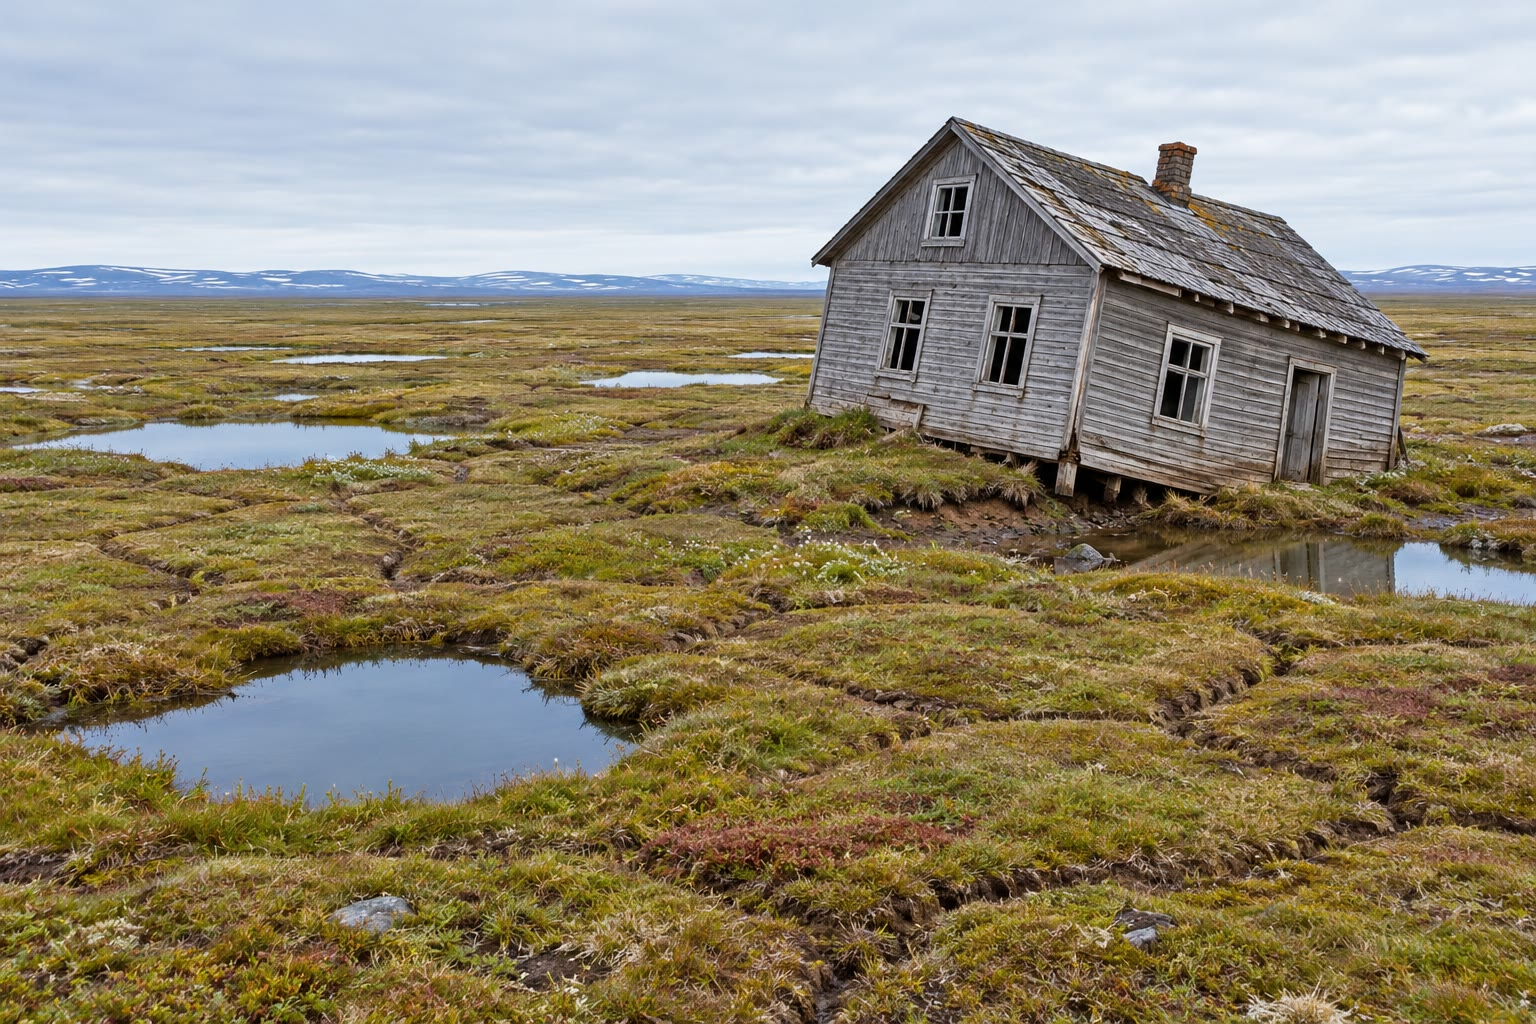
\includegraphics[width=\linewidth]{images/book1/ai/g8-permafrost-house.jpg}
\end{minipage}\hfill
\begin{minipage}[c]{0.46\linewidth}\centering
\begin{tikzpicture}[font=\footnotesize]
  \fill[omLithAlluv] (0,0) rectangle (3.2,-0.6);
  \fill[omIce!70!omLithShale] (0,-0.6) rectangle (3.2,-3.0);
  \foreach \x/\y in {0.4/-1.0, 1.5/-1.3, 2.6/-0.9, 0.9/-1.9, 2.1/-2.2, 0.5/-2.6, 2.8/-2.6}
    \fill[white] (\x,\y) ellipse (0.22 and 0.06);
  \fill[omLithShale!60] (0,-3.0) rectangle (3.2,-3.6);
  \draw[green!45!black, line width=1pt] (0,0) -- (3.2,0);
  \node[anchor=west, align=left] at (3.3,-0.3) {camada ativa:\\ descongela a cada\\ verão};
  \node[anchor=west, align=left] at (3.3,-1.8) {permafrost:\\ congelado o ano todo,\\ lentes de gelo};
  \node[anchor=west, align=left] at (3.3,-3.3) {chão não\\ congelado};
\end{tikzpicture}
\end{minipage}

\smallskip
{\small À esquerda: uma casa que se inclina sobre o \omterm{def:g8:ice-on-earth:permafrost}{permafrost} que
descongela, na tundra (ilustração de uma cena genérica feita por IA). À
direita: o chão embaixo da tundra (um esboço, fora de escala).}
\label{fig:g8:ice-on-earth:permafrost}
\end{omfigure}

\section{As glaciações}

O gelo nem sempre cobriu a mesma parte da Terra. Há cerca de \num{20000}
anos, \omterm{def:g8:ice-on-earth:ice-sheet}{mantos de gelo} cobriam boa parte da América do Norte e do norte da
Europa, inclusive a Escandinávia.
As \omterm{def:g8:ice-on-earth:glacier}{geleiras} cobriam então cerca de um quarto das terras, contra cerca de
um décimo hoje. Tanta água estava presa nesse gelo que o \omterm{def:g2:water-on-earth:ocean}{mar} ficava mais
de \qty{120}{m} abaixo do nível de hoje: partes das \omterm{def:g8:the-oceans:seafloor}{plataformas
continentais} atuais eram terra firme. A partir de cerca de \num{15000} anos atrás, os \omterm{def:g8:ice-on-earth:ice-sheet}{mantos de gelo} derreteram e recuaram, e
o \omterm{def:g2:water-on-earth:ocean}{mar} subiu; ele chegou mais ou menos ao seu nível atual há cerca de
\num{8000} anos.
% ledger: usgs:lgm, nsidc:ice-sheets, nsidc:ice-cover

\begin{definition}[Glaciação]\label{def:g8:ice-on-earth:ice-age}
Uma \emph{glaciação}\index{glaciacao@glaciação} é um longo período frio da história da Terra em que
os \omterm{def:g8:ice-on-earth:ice-sheet}{mantos de gelo} se estendem muito além das regiões polares e cobrem
grandes partes dos \omterm{def:g3:continents-and-oceans:continent}{continentes}. A última glaciação teve o seu momento mais
frio há cerca de \num{20000} anos e terminou há cerca de \num{12000} anos.
\end{definition}
% ledger: usgs:lgm, nps:u-valley

As pistas da última \omterm{def:g8:ice-on-earth:ice-age}{glaciação} estão por toda parte nas terras que ela
cobriu: \omterm{def:g8:ice-on-earth:glacial-landforms}{vales em U} longe de qualquer \omterm{def:g8:ice-on-earth:glacier}{geleira} atual, \omterm{def:g8:ice-on-earth:glacial-landforms}{morenas} frontais
atravessando \omterm{def:g1:landscapes-around-us:landform}{planícies}, blocos erráticos deitados em campos. E ela não foi
a única. Nas últimas centenas de milhares de anos, as \omterm{def:g8:ice-on-earth:ice-age}{glaciações} e as
épocas mais quentes entre elas se sucederam muitas e muitas vezes; nós
vivemos numa das épocas quentes. O \cref{ch:g9:climate-past-and-present}
conta como os cientistas leem essa longa história no próprio gelo da
Antártida.
% ledger: nps:u-valley, nps:moraines, usgs:erratic

\section{Exercícios}

\begin{exercise}[$\star$]\label{exo:g8:ice-on-earth:1}
Usando o corte longitudinal de uma \omterm{def:g8:ice-on-earth:glacier}{geleira} deste capítulo, dê o nome:
(a) da parte da \omterm{def:g8:ice-on-earth:glacier}{geleira} onde ela ganha gelo; (b) da parte onde ela perde
gelo; (c) da ponta da \omterm{def:g8:ice-on-earth:glacier}{geleira}; (d) da crista de detritos rochosos na sua
extremidade.
\end{exercise}

\begin{exercise}[$\star$]\label{exo:g8:ice-on-earth:2}
% ledger: nsidc:firn, nsidc:glacier-flow, nsidc:sea-ice-def
Verdadeiro ou falso? Corrija as frases falsas. (a) Uma \omterm{def:g8:ice-on-earth:glacier}{geleira} é feita de
água do \omterm{def:g2:water-on-earth:ocean}{mar} congelada. (b) A \omterm{def:g4:clouds-rain-snow:precipitation}{neve} leva cerca de um ano para virar firn.
(c) Quando uma \omterm{def:g8:ice-on-earth:glacier}{geleira} recua, o seu gelo sobe a encosta. (d) O \omterm{def:g8:ice-on-earth:sea-ice}{gelo
marinho} do Ártico é menor em setembro.
\end{exercise}

\begin{exercise}[$\star$]\label{exo:g8:ice-on-earth:3}
% ledger: usgs:erratic, nsidc:permafrost
Dê a palavra para cada descrição: (a) um \omterm{def:g1:landscapes-around-us:landform}{vale} de fundo largo e encostas
íngremes, escavado pelo gelo; (b) um matacão levado para longe do seu
lugar de origem por uma \omterm{def:g8:ice-on-earth:glacier}{geleira}; (c) uma placa de gelo flutuante ainda
ligada ao gelo sobre terra; (d) um chão que fica congelado durante pelo
menos dois anos seguidos.
\end{exercise}

\begin{exercise}[$\star$]\label{exo:g8:ice-on-earth:4}
% ledger: nsidc:ice-sheets, nsidc:ice-cover
(a) Que duas terras estão cobertas por \omterm{def:g8:ice-on-earth:ice-sheet}{mantos de gelo} hoje? (b) Qual das
duas faria o \omterm{def:g2:water-on-earth:ocean}{mar} subir mais se todo o seu gelo derretesse, e quanto?
(c) Que parte das terras da Terra está coberta de gelo hoje?
\end{exercise}

\begin{exercise}[$\star\star$]\label{exo:g8:ice-on-earth:5}
% ledger: data:b1-nsidc-sea-ice (figdata/grade-8/sea_ice.py)
Use o gráfico do \omterm{def:g8:ice-on-earth:sea-ice}{gelo marinho} do Ártico em setembro. (a) Leia a extensão
em 1979 e em 2012. (b) Quantos milhões de~km$^2$ ela diminuiu entre esses
dois anos? (c) Que fração da extensão de 1979 tinha desaparecido em 2012?
Arredonde para uma fração simples. (d) Por que é mais confiável comparar a
linha de tendência do que dois anos isolados?
\end{exercise}

\begin{exercise}[$\star\star$]\label{exo:g8:ice-on-earth:6}
% ledger: nsidc:muir, uw:pedersen
A extremidade da \omterm{def:g8:ice-on-earth:glacier}{geleira} Muir recuou \qty{12}{km} entre 1941 e 2004.
(a) Quantos anos são? (b) Qual foi o seu recuo médio por ano, em metros?
Arredonde para a dezena de metros mais próxima. (c) A \omterm{def:g8:ice-on-earth:glacier}{geleira} Pedersen
recuou \qty{3.2}{km} entre 1984 e 2021. Qual foi o seu recuo médio por
ano? (d) Que \omterm{def:g8:ice-on-earth:glacier}{geleira} recuou mais depressa?
\end{exercise}

\begin{exercise}[$\star\star$]\label{exo:g8:ice-on-earth:7}
Explique, em algumas frases e em ordem, como a \omterm{def:g4:clouds-rain-snow:precipitation}{neve} que cai no alto de uma
\omterm{def:g1:landscapes-around-us:landform}{montanha} vira o gelo da extremidade de uma \omterm{def:g8:ice-on-earth:glacier}{geleira}, bem abaixo no \omterm{def:g1:landscapes-around-us:landform}{vale}.
Use as palavras \emph{firn}, \emph{zona de acumulação}, \emph{desce} e
\emph{zona de ablação}.
\end{exercise}

\begin{exercise}[$\star\star$]\label{exo:g8:ice-on-earth:8}
% ledger: nsidc:ice-shelves
Dois copos estão cheios até o mesmo nível. No copo A, cubos de gelo
flutuam na água; no copo B, os mesmos cubos de gelo estão sobre uma pedra,
acima da água. (a) Depois que o gelo derrete, em que copo o nível subiu?
(b) Que copo é um modelo de um \omterm{def:g8:ice-on-earth:ice-sheet}{iceberg} que derrete no \omterm{def:g2:water-on-earth:ocean}{mar}? E de um \omterm{def:g8:ice-on-earth:ice-sheet}{manto
de gelo} que derrete sobre a terra? (c) Por que a quebra de uma \omterm{def:g8:ice-on-earth:ice-sheet}{plataforma
de gelo} ainda importa para o \omterm{def:g4:world-physical-map:altitude}{nível do mar}?
\end{exercise}

\begin{exercise}[$\star\star$]\label{exo:g8:ice-on-earth:9}
Uma caminhante atravessa um \omterm{def:g1:landscapes-around-us:landform}{vale} largo, de fundo plano e encostas muito
íngremes. No meio de um campo, ela encontra um matacão de granito do
tamanho de um carro; todas as \omterm{def:g3:stones-pebbles-sand:rock}{rochas} do \omterm{def:g1:landscapes-around-us:landform}{vale} são calcário. Mais acima, uma
longa crista de pedras misturadas corre ao longo da encosta do \omterm{def:g1:landscapes-around-us:landform}{vale}.
(a) Que forma tem o \omterm{def:g1:landscapes-around-us:landform}{vale}, e o que o escavou? (b) Como o matacão chegou
ali? Como ele se chama? (c) O que é a crista, e o que a sua altura na
encosta do \omterm{def:g1:landscapes-around-us:landform}{vale} lhe diz?
\end{exercise}

\begin{exercise}[$\star\star$]\label{exo:g8:ice-on-earth:10}
% ledger: nsidc:ice-sheets
O \omterm{def:g8:ice-on-earth:ice-sheet}{manto de gelo} da Antártida faria o \omterm{def:g2:water-on-earth:ocean}{mar} subir cerca de \qty{58}{m} se
derretesse inteiro, e o \omterm{def:g8:ice-on-earth:ice-sheet}{manto de gelo} da Groenlândia, cerca de
\qty{7.4}{m}. (a) Quanto um décimo do gelo da Groenlândia acrescentaria?
(b) Quanto um centésimo do gelo da Antártida acrescentaria? (c) Quantas
vezes mais a Antártida guarda que a Groenlândia? Arredonde para o número
inteiro mais próximo.
\end{exercise}

\begin{exercise}[$\star\star\star$]\label{exo:g8:ice-on-earth:11}
% ledger: data:b1-nsidc-sea-ice (figdata/grade-8/sea_ice.py: mean_1980s, mean_2010s, trend)
A extensão média do \omterm{def:g8:ice-on-earth:sea-ice}{gelo marinho} do Ártico em setembro foi de
\num{7.21}~milhões~de~\unit{km^2} nos anos 1980--1989 e de
\num{4.65}~milhões~de~\unit{km^2} nos anos 2010--2019. (a) Um milhão é
$10^6$. Escreva os dois valores em km$^2$, sem a palavra ``milhões''.
(b) Quanto a extensão média diminuiu entre essas duas décadas?
(c) As duas décadas estão a 30 anos uma da outra. Qual é a diminuição por
década? Compare com os \num{0.76}~milhão~de~\unit{km^2} por década da linha de tendência.
(d) Por que uma linha de tendência reta não pode ser prolongada para
sempre no futuro?
\end{exercise}

\begin{exercise}[$\star\star\star$]\label{exo:g8:ice-on-earth:12}
% ledger: usgs:lgm (the shelf slope is exercise data)
Há cerca de \num{20000} anos, o \omterm{def:g2:water-on-earth:ocean}{mar} ficava cerca de \qty{120}{m} abaixo
do nível de hoje. Ao largo de um \omterm{def:g1:landscapes-around-us:water}{litoral}, a \omterm{def:g8:the-oceans:seafloor}{plataforma continental} desce
muito suavemente, \qty{1}{m} a cada \qty{1}{km} \omterm{def:g2:water-on-earth:ocean}{mar} adentro (dados de
exercício). (a) A que distância \omterm{def:g2:water-on-earth:ocean}{mar} adentro ficava o \omterm{def:g1:landscapes-around-us:water}{litoral} nessa época?
(b) Para onde foi a água dos \qty{120}{m} que faltavam? (c) Explique por
que uma \omterm{def:g8:ice-on-earth:glacial-landforms}{morena} frontal encontrada hoje numa \omterm{def:g1:landscapes-around-us:landform}{planície}, longe de qualquer
\omterm{def:g1:landscapes-around-us:landform}{montanha}, é uma pista da mesma \omterm{def:g8:ice-on-earth:ice-age}{glaciação}.
\end{exercise}

\section{Problema: O longo recuo de uma geleira}

\begin{problem}[{Problema de fim de semana --- a extremidade de uma
geleira de montanha foi medida a cada dez anos desde 1960; calcula-se a
sua velocidade de recuo, e lê-se o vale que ela deixa}]
\label{pb:g8:ice-on-earth:1}
% ledger: nsidc:muir, uw:pedersen, nps:moraines (figdata/grade-8/glacier_retreat.py; Glacier G and its measurements are exercise data)
A cada dez anos desde 1960, uma equipe mede a posição da extremidade da
\omterm{def:g8:ice-on-earth:glacier}{Geleira}~G, uma \omterm{def:g8:ice-on-earth:glacier}{geleira} de \omterm{def:g1:landscapes-around-us:landform}{vale} nas \omterm{def:g1:landscapes-around-us:landform}{montanhas}. A distância é medida \omterm{def:g1:landscapes-around-us:landform}{vale}
acima a partir de um marco de pedra~R, pintado no fundo do \omterm{def:g1:landscapes-around-us:landform}{vale} na
extremidade, em 1960. Um refúgio~H fica ao lado do fundo do \omterm{def:g1:landscapes-around-us:landform}{vale},
\qty{1980}{m} \omterm{def:g1:landscapes-around-us:landform}{vale} acima a partir de~R. O \omterm{def:g2:drawing-to-map:map}{mapa} mostra a extremidade em
cada medição e a crista logo abaixo da extremidade de 1960.

\begin{center}
\begin{tikzpicture}
\begin{axis}[axis equal image, width=12.5cm, xmin=-500, xmax=2600, ymin=-760, ymax=760,
  axis lines=none, clip=true]
  \fill[black!13] (axis cs:-500,-760) rectangle (axis cs:2600,760);
  \addplot[fill=white, draw=none] table[x=y, y=x] {figdata/out/grade-8-glacier_retreat-floor.dat} -- cycle;
  \addplot[fill=omIce, draw=none] table[x=y, y=x] {figdata/out/grade-8-glacier_retreat-ice.dat} -- cycle;
  \addplot[black!70, line width=0.8pt] table[x=y, y=x] {figdata/out/grade-8-glacier_retreat-walls.dat};
  \addplot[omCold, line width=0.9pt] table[x=y, y=x] {figdata/out/grade-8-glacier_retreat-fronts.dat};
  \addplot[omLithCongl!80!black, line width=3pt] table[x=y, y=x] {figdata/out/grade-8-glacier_retreat-moraine.dat};
  \addplot[only marks, mark=none, nodes near coords, point meta=explicit symbolic,
    every node near coord/.style={anchor=south, rotate=90, font=\scriptsize, inner sep=1pt}]
    table[x=y, y=x, meta=year] {figdata/out/grade-8-glacier_retreat-labels.dat};
  \addplot[only marks, mark=*, mark size=2pt] coordinates {(0,0)};
  \node[font=\footnotesize\bfseries, anchor=south east] at (axis cs:-10,10) {R};
  \addplot[only marks, mark=square*, mark size=2.6pt, omDef] coordinates {(1980,-560)};
  \node[font=\footnotesize\bfseries, anchor=north] at (axis cs:1980,-590) {H};
  \node[font=\scriptsize, anchor=west] at (axis cs:-480,-590) {vale acima $\longrightarrow$};
  \node[font=\scriptsize] at (axis cs:2250,0) {gelo em 2020};
  \draw[black, line width=1.2pt] (axis cs:2000,640) -- (axis cs:2500,640)
    node[midway, below, font=\scriptsize] {\qty{500}{m}};
\end{axis}
\end{tikzpicture}

\smallskip
{\small
\begin{tabular}{|l|c|c|c|c|c|c|c|}
\hline
ano & 1960 & 1970 & 1980 & 1990 & 2000 & 2010 & 2020 \\
\hline
distância da extremidade a R (m) & 0 & 180 & 330 & 520 & 700 & 880 & 1080 \\
\hline
\end{tabular}}
\end{center}

\noindent\textbf{Parte I --- As posições da extremidade.}\par\nopagebreak
\begin{enumerate}[beginpenalty=10000]
  \item Quanto a extremidade recuou entre 1960 e 2020?
  \item Calcule quanto ela recuou em cada década. Em que década ela recuou
        menos? E mais?
  \item A \omterm{def:g8:ice-on-earth:glacier}{geleira} parou de descer a encosta? Explique.
  \item A crista escura logo abaixo da extremidade de 1960 é feita de
        detritos rochosos misturados. Como ela se chama, e como se formou?
\end{enumerate}

\noindent\textbf{Parte II --- A velocidade de recuo.}\par\nopagebreak
\begin{enumerate}[resume, beginpenalty=10000]
  \item Qual foi o recuo médio por década entre 1960 e 2020?
  \item E por ano?
  \item A \omterm{def:g8:ice-on-earth:glacier}{geleira} Muir recuou \qty{12}{km} em 63 anos, cerca de
        \qty{190}{m} por ano. Quantas vezes isso foi mais rápido que a
        \omterm{def:g8:ice-on-earth:glacier}{Geleira}~G?
  \item A \omterm{def:g8:ice-on-earth:glacier}{Geleira}~G ganhou mais gelo na sua zona de acumulação do que
        perdeu na sua zona de ablação, ou menos? Explique.
\end{enumerate}

\noindent\textbf{Parte III --- O vale que ela deixa.}\par\nopagebreak
\begin{enumerate}[resume, beginpenalty=10000]
  \item Que forma você esperaria que o fundo do \omterm{def:g1:landscapes-around-us:landform}{vale} entre R e a
        extremidade de 2020 tivesse em corte transversal? Por quê?
  \item Em 2020, a que distância a extremidade estava do nível do refúgio?
  \item Na velocidade média da Parte~II, de quantos anos a extremidade
        precisaria para chegar ao nível do refúgio? Em que ano isso seria?
  \item Dê uma razão pela qual esse ano não é uma previsão.
\end{enumerate}
\end{problem}
